\subsection{Frozen synthetic evaluation}

The completed matrix contains 1,260 attempts and no failed cells. The predefined synthetic disposition is \textbf{SUPPORTED}. Across the primary conditions, the mean paired seed-level relative MSE change is -36.01\% (95\% bootstrap interval [-38.04, -34.00]\%). Mean weight-update reduction is 58.55\%. These quantities use the frozen aggregation rule; the table below reports pooled means over the same balanced conditions.

\begin{table}[ht]\centering\small\begin{tabular}{lrrrr}\toprule Method & MSE & Updates & Arithmetic & State bytes\\\midrule

Always-update bank & 0.4445 & 953.6 & 974385 & 5456 \\

RLS baseline & 0.5378 & 953.6 & 798925 & 3280 \\

Memory gate & 0.3426 & 395.2 & 499856 & 5456 \\

Capacity 1 & 0.5411 & 875.4 & 758486 & 3504 \\

Frozen zero & 1.0097 & 0.0 & 26074 & 1992 \\

FIFO kNN & 0.9124 & 0.0 & 981053 & 5576 \\

No bank (RLS) & 0.5378 & 953.6 & 798925 & 3280 \\

FIFO replay & 1.0540 & 1906.2 & 173286 & 5576 \\

Uniform bank & 1.0036 & 395.2 & 499856 & 5456 \\

\bottomrule\end{tabular}\caption{Primary-condition means over 100 task instances per method. State is maximum numerical state, not process RSS.}\end{table}

\begin{figure}[ht]\centering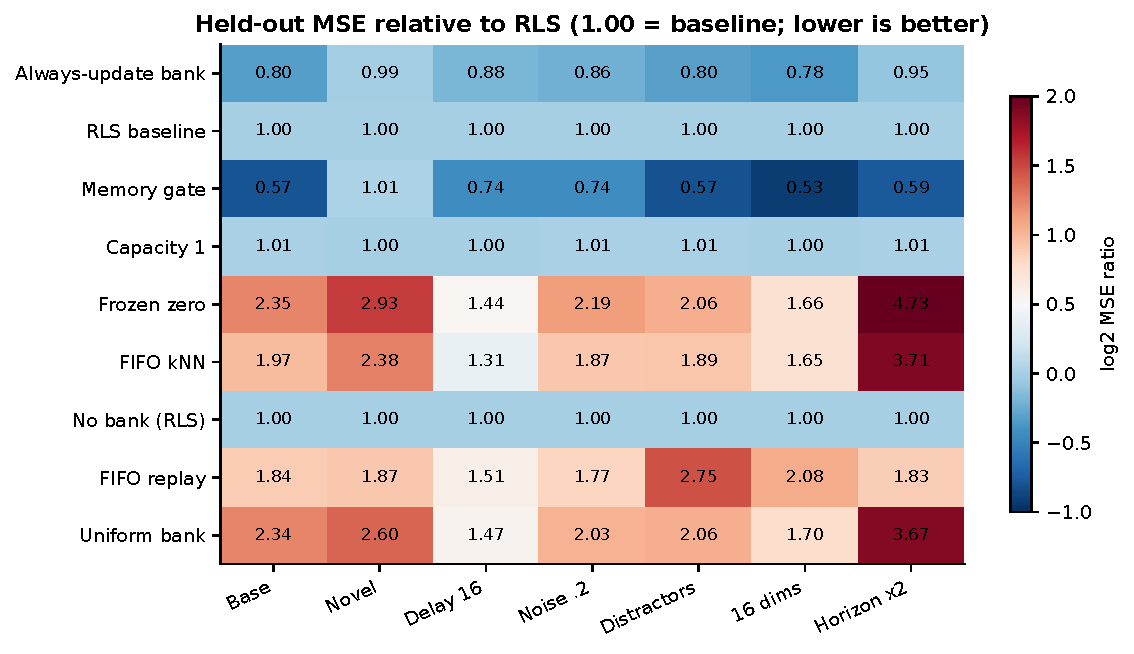
\includegraphics[width=\linewidth]{figures/condition_heatmap.pdf}\caption{Complete condition matrix. Values are mean-MSE ratios, not paired-effect confidence bounds.}\end{figure}

\begin{figure}[ht]\centering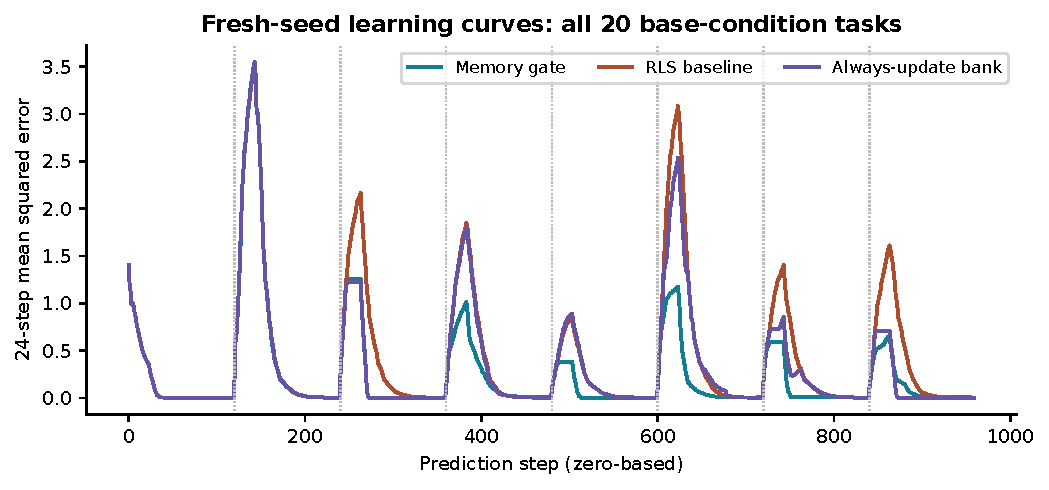
\includegraphics[width=\linewidth]{figures/learning_curves.pdf}\caption{Rolling errors averaged over all 20 fresh base-condition seeds. Vertical lines mark generator changes, hidden from the learner.}\end{figure}

Against the all-update bank, the candidate relative MSE change is -22.66\% (95\% interval [-24.65, -20.73]\%). This comparison is descriptive mechanism evidence and is distinct from the primary baseline test.

\begin{figure}[ht]\centering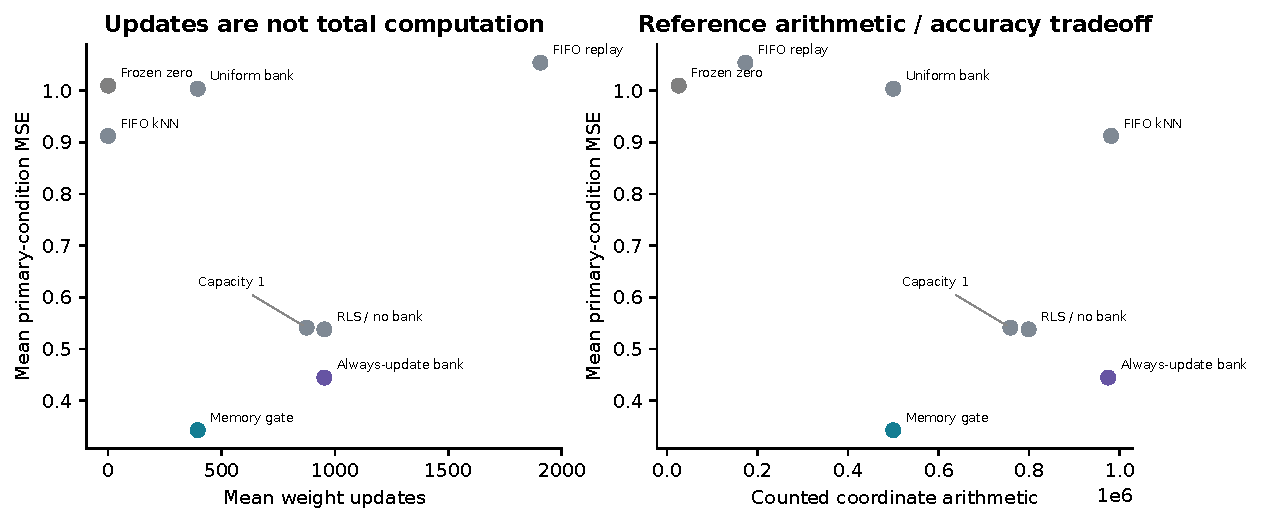
\includegraphics[width=\linewidth]{figures/efficiency.pdf}\caption{Accuracy versus actual update counts and counted arithmetic. Additional prediction work can offset gradient savings.}\end{figure}

\subsection{Chronological real-data transfer}

All ten registered methods were attempted. Six RLS-based methods failed because the covariance update lost positive definiteness: the candidate, baseline, all-update bank, capacity-one bank, uniform bank, and no-bank RLS. The candidate failed after 6,702 predictions; the baseline failed after 710, before the test boundary. Their partial errors are not substitutes for a full-transfer comparison. Four controls completed, each scoring 4,668 test targets. Real-transfer efficacy is therefore \textbf{not established}. The overall evidence disposition is \textbf{MIXED}: supported on the registered synthetic endpoint, with a numerical failure preventing the real-data comparison.

\begin{table}[ht]\centering\small\begin{tabular}{lrr}\toprule Method & CO MSE & Test updates\\\midrule

Always-update bank & FAILED & --- \\

RLS baseline & FAILED & --- \\

Memory gate & FAILED & --- \\

Capacity 1 & FAILED & --- \\

Frozen zero & 7.606414 & 0 \\

FIFO kNN & 0.913742 & 0 \\

Last observation & 3.228987 & 0 \\

No bank (RLS) & FAILED & --- \\

FIFO replay & 0.551697 & 9336 \\

Uniform bank & FAILED & --- \\

\bottomrule\end{tabular}\caption{All real-transfer methods, including a last-observation control.}\end{table}

\begin{figure}[ht]\centering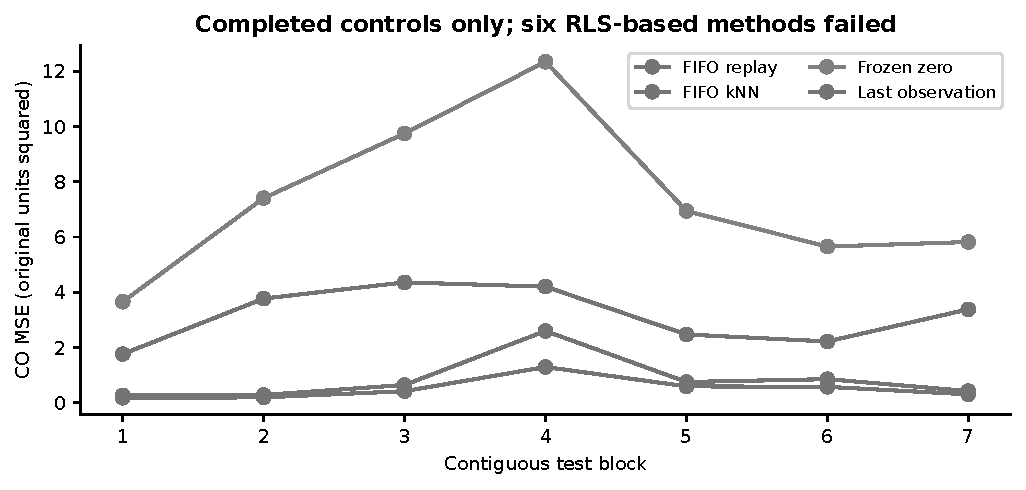
\includegraphics[width=\linewidth]{figures/real_transfer.pdf}\caption{Seven contiguous temporal blocks are descriptive, not independent replications.}\end{figure}

\subsection{Evidence boundary}

These are executed local CPU results. Kaggle execution and independent external replication are separate release gates; this manuscript does not infer them from the presence of a notebook or package. The v1 protected evaluation remains untouched.
